\documentclass{beamer}

%\mode<presentation>
%{
%  \usetheme{Warsaw}
%  \setbeamercovered{transparent}
%}

\usepackage{amsmath}
\usepackage[english]{babel}
\usepackage[latin1]{inputenc}
\usepackage{graphicx}
\usepackage{csquotes}
\usepackage{times}
\usepackage[T1]{fontenc}
\usepackage{bm}
\usepackage[
  backend=biber,
  citestyle=authoryear,
  url=false
]{biblatex}
\usepackage{tikz}
\usepackage{pgfplots,pgfplotstable}
\usepackage{siunitx}

\addbibresource{refs.bib}

\graphicspath{{figures/}}

\usetikzlibrary{external}
\usetikzlibrary{matrix}
\usetikzlibrary{positioning}

\tikzexternalize[prefix=tikz/]
\pgfplotstableset{col sep=comma}

\tikzset{
  every edge/.append style={thick},
  afm/.style={red!80!black},
  fm/.style={blue},
  spin/.style={-latex,very thick},
  site/.style={inner sep=2pt,outer sep=4pt,node distance=0.5cm},
  region/.style={rectangle,draw,thick,fill=gray!20,node distance=0.5cm,minimum
    width=#1,minimum height=#1},
  declare function={
    gauss(\x,\pos,\sigma) =
    1/(sqrt(2*pi)*\sigma)*exp(-(\x-\pos)^2/(2*\sigma^2));}
}

\pgfplotsset{
  compat=newest,
  every axis/.append style={
    axis line style={thick,gray},
    xlabel near ticks,
    ylabel near ticks,
    mark options={fill opacity=0.4}
  },
  every axis plot post/.append style={thick},
  sketch plots/.style={
    clip=false,
    axis lines=center,
    every axis plot post/.append style={mark=none},
  },
  label at end/.style={
    every axis x label/.style={at=(current axis.right of origin),anchor=west},
    every axis y label/.style={at=(current axis.above origin),anchor=south},
  },
  with y errors/.style={
    error bars/y dir=both,
    error bars/y explicit
  }
}


\newcommand{\abs}[1]{\left|#1\right|}
\newcommand{\av}[1]{\left<#1\right>}
\newcommand{\cbr}[1]{\left\{#1\right\}}
\newcommand{\del}[1]{\left(#1\right)}
\newcommand{\sbr}[1]{\left[#1\right]}
\newcommand{\dav}[1]{\sbr{#1}_{\text{av}}}
\newcommand{\ham}{\mathcal{H}}
\newcommand{\dif}{\mathop{}\!d}
\newcommand{\qea}{q_{\text{EA}}}

\newcommand{\spinup}[1][6pt]{\tikz{\draw[spin] (0,-#1) -- (0, #1);}}
\newcommand{\spindn}[1][6pt]{\tikz{\draw[spin] (0, #1) -- (0,-#1);}}

\renewcommand{\vec}[1]{\bm{#1}}


\title[Nature of the spin-glass phase]{
  Nature of the spin-glass phase in models with long-range interactions
}

%\subtitle{Presentation Subtitle}

\author{Matt Wittmann}

\institute[UC Santa Cruz] % (optional, but mostly needed)
{
  Physics Department\\
  University of California, Santa Cruz
}

\date[]{Defense talk\\September 2015\\Peter Young, advisor}

\subject{Talks}

% \pgfdeclareimage[height=0.5cm]{university-logo}{university-logo-filename}
% \logo{\pgfuseimage{university-logo}}

\AtBeginSection[]
{
  \begin{frame}<beamer>{Overview}
    \tableofcontents[currentsection]
  \end{frame}
}

%\beamerdefaultoverlayspecification{<+->}


\begin{document}

\begin{frame}
  \titlepage
\end{frame}

\begin{frame}{Overview}
  \tableofcontents%[pausesections]
\end{frame}

\section{Introduction}

\subsection{What is a spin glass?}

\begin{frame}[fragile]{What is a spin glass?}
  \centering
  Magnet with \alert{frustration} and \alert{quenched disorder}\dots
  \begin{columns}[b]
    \column{0.5\textwidth}
    \begin{figure}
      \centering
      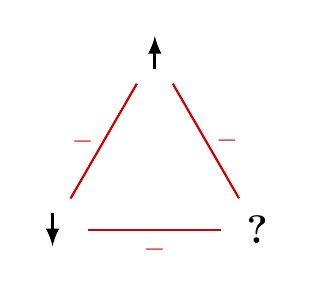
\begin{tikzpicture}
        \def\r{1.5cm}
        \node [site,circle] (1) at ( 90:\r) {\spinup};
        \node [site,circle] (2) at (210:\r) {\spindn} edge[afm] node[left] {$-$} (1);
        \node [site,circle] (3) at (330:\r) {\Large{\textbf{\alert{?}}}}
          edge[afm] node[below] {$-$} (2)
          edge[afm] node[right] {$-$} (1);
      \end{tikzpicture}
    \end{figure}
    \column{0.5\textwidth}
    \begin{figure}
      \centering
      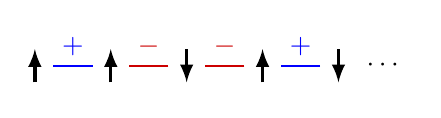
\begin{tikzpicture}
        \def\spinlen{4pt}
        \node (1) [site] {\spinup};
        \node (2) [site,right=of 1] {\spinup}
          edge[fm] node [above] {$+$} (1);
        \node (3) [site,right=of 2] {\spindn}
          edge[afm] node [above] {$-$} (2);
        \node (4) [site,right=of 3] {\spinup}
          edge[afm] node [above] {$-$} (3);
        \node (5) [site,right=of 4,label=right:$\cdots$] {\spindn}
          edge[fm] node [above] {$+$} (4);
      \end{tikzpicture}
      \vskip 1.2cm
    \end{figure}
  \end{columns}
\end{frame}

\begin{frame}{Edwards-Anderson $\pm J$ model}
  \begin{itemize}
    \item Ising-like Hamiltonian
      \begin{equation*}
        \ham = -\frac{1}{2} \sum_{ij} J_{ij} S_i S_j
      \end{equation*}
    \item Nearest neighbor interactions \alert{quenched, random} variables
      \begin{equation*}
        P(J_{ij}) =
        \begin{cases}
          \frac{1}{2} \delta(J_{ij}-J) +
          \frac{1}{2} \delta(J_{ij}+J) &
          \text{$i$, $j$ nearest neighbors} \\
          0 & \text{otherwise}
        \end{cases}
      \end{equation*}
    \item Disorder and \emph{frustration}, \textit{e.g.}\quad
      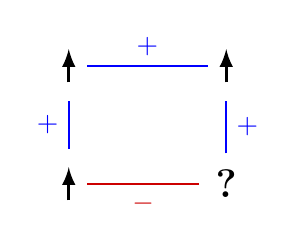
\begin{tikzpicture}[x={(2,0)},y={(0,1.5)},baseline=(current bounding box.center)]
        \node [site] (1) at (1,1) {\spinup};
        \node [site] (2) at (0,1) {\spinup} edge[fm] node[above] {$+$} (1);
        \node [site] (3) at (0,0) {\spinup} edge[fm] node[left]  {$+$} (2);
        \node [site] (4) at (1,0) {\Large\textbf{\alert{?}}}
          edge[afm] node[below] {$-$} (3)
          edge[fm]  node[right] {$+$} (1);
      \end{tikzpicture}
  \end{itemize}
\end{frame}

\begin{frame}[fragile]{Laboratory spin glasses}
  \begin{columns}
    \column{0.5\textwidth}
    \begin{itemize}
      \item Original examples: alloys of nonmagnetic metals with magnetic
        impurities \textit{e.g.} Au$_{1-x}$Fe$_x$, Cu$_{1-x}$Mn$_x$
      \item Spatial disorder + \alert{RKKY~interaction\footnotemark}
        \begin{equation*}
          J(r) \propto \frac{\cos(2 k_F r)}{r^3}
        \end{equation*}
    \end{itemize}
    \column{0.5\textwidth}
    \begin{figure}
      \begin{tikzpicture}
        \begin{axis}[
          name=plot,
          sketch plots,
          label at end,
          width=\columnwidth,
          xlabel={$r$},
          ylabel={$J(r)$},
          ticks=none,
          axis y line=left,
          domain=1:4,
          smooth,
          enlargelimits
        ]
          \addplot+[smooth] {cos(deg(2*pi*x))/x^3};
        \end{axis}
        \def\site{\draw [blue] (0,0) circle (1.2pt);}
        \def\spin{
          \draw [red] (0,0) circle (1.2pt);
          \draw [red,->] (0,-0.08) -- (0,0.12);}
        \node at (plot.north east) [
          matrix,
          draw,
          anchor=north east,
          column sep=5pt,
          row sep=5pt,
        ]{
          \site & \site & \spin & \site & \site & \site & \spin & \site \\
          \site & \site & \site & \site & \site & \spin & \site & \site \\
          \site & \spin & \site & \site & \site & \site & \site & \site \\
          \site & \site & \site & \site & \site & \site & \site & \spin \\
        };
      \end{tikzpicture}
    \end{figure}
  \end{columns}
  \footnotetext{Ruderman, Kittel, Kasuya, and Yosida}
\end{frame}

\begin{frame}{Evidence of phase transition}
  \begin{columns}
    \column{0.5\textwidth}
    \begin{itemize}
      \item \textcite{cannella1972magnetic}
      \item Au$_{1-x}$Fe$_x$
      \item Cusp in ac susceptibility
      \item Temperature of peak and height found to vary with $x$
      \item No singular behavior of specific heat
    \end{itemize}
    \column{0.5\textwidth}
    \includegraphics[width=\columnwidth]{ac-susc}
  \end{columns}
\end{frame}

\begin{frame}{Other examples}
  \begin{columns}
    \column{0.5\textwidth}
    \begin{itemize}
      \item ``Vortex-glass'' transition in high-$T_c$ superconductors
      \item Networks: neural, social, communications, etc.
      \item Deep connection with optimization problems,
        \textit{e.g.} 3-SAT, TSP, \dots
    \end{itemize}
    \column{0.5\textwidth}
    \includegraphics[width=\columnwidth]{TSP}
  \end{columns}
\end{frame}


\subsection{Behavior of spin glasses}

\begin{frame}{Features of spin glasses}
  \begin{itemize}
    \item \alert{Complex energy landscape}
    \item Many metastable states, large valleys
    \item \alert{Slow dynamics}
    \item Unique nonequilibrium effects (\textit{e.g.} aging, memory)
    \item Finding the ground state is (NP-) hard%
      \footnote{\textcite{barahona1982computational}}
  \end{itemize}
  \centering
  \begin{figure}
    \begin{tikzpicture}
      \begin{axis}[
        width=\columnwidth,height=0.4\columnwidth,
        xlabel={configuration},ylabel={$E$},
        ticks=none,
        axis lines=left,
        enlarge x limits=false,
        enlarge y limits=true
      ]
        \addplot+[smooth,mark=none] file {pinknoise.dat};
      \end{axis}
    \end{tikzpicture}
  \end{figure}
\end{frame}


\subsection{Spin-glass models}

\begin{frame}{Edwards-Anderson model}
  \begin{itemize}
    \item \textcite{edwards1975theory}: competition between FM and AFM interactions
      is the essential physics
    \item Ising-like model with \alert{short-range} interactions
      \begin{equation*}
        \ham = -\frac{1}{2} \sum_{ij} J_{ij} S_i S_j
      \end{equation*}
    \item Interactions $J_{ij}$ are quenched, Gaussian random variables with
      zero mean
      \begin{equation*}
        P(J_{ij})=
        \begin{cases}
          \frac{1}{\sqrt{2\pi}} e^{-J_{ij}^2/2} &
          \text{$i$, $j$ nearest neighbors} \\
          0 & \text{otherwise}
        \end{cases}
      \end{equation*}
    \item Simple-looking model with \alert{frustration} and \alert{disorder}
  \end{itemize}
\end{frame}

\begin{frame}{Spin-glass phase transition}
  \alert{What is an appropriate order parameter for spin glasses?}
  \begin{itemize}
    \item Magnetization vanishes at all temperatures (symmetry)
    \item Consider thermal average of a single spin
      \begin{equation*}
        \av{S_i}=
        \begin{cases}
          0 & T > T_c \\
          \text{\alert{finite}} & T < T_c \quad \text{(SG phase)}
        \end{cases}
      \end{equation*}
    \item \textcite{edwards1975theory} define
      \begin{equation*}
        \qea \equiv \lim_{N\to\infty} \frac{1}{N} \sum_i \av{S_i}^2
      \end{equation*}
    \item Does \alert{not} distinguish broken-symmetry states
  \end{itemize}
  EA model difficult to study analytically ($d_l>2$). First approximation is
  \alert{mean-field theory}\dots
\end{frame}

\begin{frame}{Sherrington-Kirkpatrick model}
  \begin{itemize}
    \item EA model $+$ infinite-range interactions $=$ SK  model
    \begin{equation*}
      P(J_{ij}) =
      \frac{1}{\sqrt{2\pi\sigma^2}} e^{-J_{ij}^2/(2\sigma^2)},\qquad
      \sigma^2 = \frac{1}{N}
    \end{equation*}
    \item Solution requires average over disorder
    \begin{equation*}
      -\beta\dav{F}=
      \dav{\log Z} \equiv
      \int\prod_{ij}\sbr{\dif J_{ij}\,P(J_{ij})} \log Z(\vec{J})
    \end{equation*}
    \item SK solve using \alert{``replica trick''}
    \begin{equation*}
      \log Z = \lim_{n \to 0} \frac{Z^n - 1}{n}
    \end{equation*}
  \end{itemize}
\end{frame}

\begin{frame}{Replica-symmetric solution}
  \begin{itemize}
    \item Effective Hamiltonian couples replicas
      \begin{equation*}
        e^{-\beta\ham_n}=
        \dav{e^{-\beta\sum_{\alpha=1}^n \ham\del{\cbr{S^{\alpha}},\cbr{J_{ij}}}}}
      \end{equation*}
    \item Solution of SK is ``replica-symmetric''
    \item Transition temperature
      \begin{equation*}
        \del{T_c^{\text{MF}}}^2 = \sum_j \dav{J_{ij}^2}
      \end{equation*}
  \end{itemize}
  But SK solution has problems: disagreement with simulation for $T<T_c$,
  \alert{negative} entropy at zero temperature\dots
\end{frame}

\begin{frame}{Replica symmetry breaking}
  \begin{itemize}
    \item Replica-symmetric solution \alert{unstable} below $T_c$
    \item \textcite{parisi1979infinite} gave correct stable solution,
      requiring ``replica symmetry breaking'' (RSB)
    \item \emph{Many} pure states below $T_c$
    \item Infinite number of order parameters,
      \begin{equation*}
        q_{\alpha\beta} = \frac{1}{N} \sum_i \av{S_i}_{\alpha} \av{S_i}_{\beta},
      \end{equation*}
      corresponding to \alert{overlaps} of pure states
      \begin{equation*}
        q_{\alpha\alpha}=\qea,\quad
        -\qea < q_{\alpha\beta} < \qea
        \quad\text{($\alpha\neq\beta$)}
      \end{equation*}
  \end{itemize}
\end{frame}

\begin{frame}[fragile]{RSB overlap distributions}
  Spin overlap of two copies:
  $q \equiv \frac{1}{N} \sum_{i=1}^N \av{S_i}_1 \av{S_i}_2$
  \begin{columns}[T]
    \column{0.5\textwidth}%
    \begin{figure}
      \begin{tikzpicture}
        \pgfmathsetmacro{\x}{0.6}
        \pgfmathsetmacro{\y}{0.9}
        \def\deltapair#1#2{(-#1*\x, #2*\y) (#1*\x, #2*\y)}
        \begin{axis}[
          sketch plots,
          label at end,
          width=\columnwidth,
          height=0.6\columnwidth,
          xmin=-1,xmax=1,
          ymin=0,ymax=1,
          xtick={-\x,\x},
          xticklabels={$-\qea$,$+\qea$},
          xtick align=outside,
          ytick=\empty,
          xlabel={$q$},
          ylabel={$P_{\mathcal{J}}(q)$},
          enlarge y limits=false,
        ]
          \addplot+[ycomb] coordinates {
            \deltapair{1}{1}
            \deltapair{0.7}{0.4}
            \deltapair{0.3}{0.5}
            \deltapair{0.1}{0.2}
          };
        \end{axis}
      \end{tikzpicture}
      Sample overlap distribution has many pairs of peaks
    \end{figure}
    \column{0.5\textwidth}
    \begin{figure}
      \begin{tikzpicture}
  \pgfmathsetmacro{\x}{0.6}
  \pgfmathsetmacro{\y}{0.9}
  \pgfmathsetmacro{\a}{0.1}
  \pgfmathsetmacro{\b}{0.6}
  \begin{axis}[
    sketch plots,label at end,
    width=\columnwidth,
    height=0.6\columnwidth,
    xmin=-1,xmax=1,
    ymin=0,ymax=1,
    xtick={-\x,\x},
    xticklabels={$-\qea$,$+\qea$},
    xtick align=outside,
    ytick=\empty,
    xlabel={$q$}, ylabel={$P(q)$},
    enlarge y limits=false,
    every axis plot post/.append style={red}
  ]
    \addplot+[ycomb,forget plot] coordinates {(-\x,\y) (\x,\y)};
    \addplot+[domain=-\x:\x] {\a + \b*x^2};
  \end{axis}
\end{tikzpicture}

      Sample-averaged distribution nonzero between $\pm\qea$
    \end{figure}
  \end{columns}
  \vfill
  Parisi's RSB solution is correct for the SK model, but

  \alert{does it also provide an accurate description of ``realistic''
    (short-range) spin glasses?}
\end{frame}



\section{Connection between dynamics and statics}


\subsection{Ergodicity breaking}

\begin{frame}{Ergodicity breaking}
  \begin{itemize}
    \item Time average (what we observe)
      \begin{equation*}
        \av{A} \equiv 
        \lim_{t\to\infty} \frac{1}{t}
        \int_0^t \dif t^{\prime} A\sbr{\vec{q}(t^{\prime})}
      \end{equation*}
    \item Equivalent to ensemble average (what we calculate)?
    \item \alert{Ergodic hypothesis}
      \begin{equation*}
        \av{A} = \int \prod_i \dif q_i\,P_{\text{eq}}(\vec{q}) A(\vec{q})
      \end{equation*}
    \item Averages are \emph{not} equivalent, \textit{e.g.} when a symmetry is
      spontaneously broken\dots
  \end{itemize}
\end{frame}

\begin{frame}[fragile]{Ergodicity breaking: ferromagnet}
  \begin{columns}
    \column{0.6\textwidth}
    \begin{itemize}
      \item For $T<T_c$, system chooses either ``up'' or ``down'', finite $\abs{M}$
      \item States have \alert{infinite lifetime} in $N\to\infty$ limit,
        \begin{equation*}
          \tau \sim \exp\sbr{N^{(d-1)/d}}
        \end{equation*}
      \item System is trapped in one or the other region of configuration space
      \item Average over \emph{all} configurations gives $M=0$\dots
      \item Can ``select'' state with nonzero field $H$, then take $H \to 0$
        \emph{after} $N \to \infty$
    \end{itemize}
    \column{0.4\textwidth}
    \begin{figure}
      \centering
      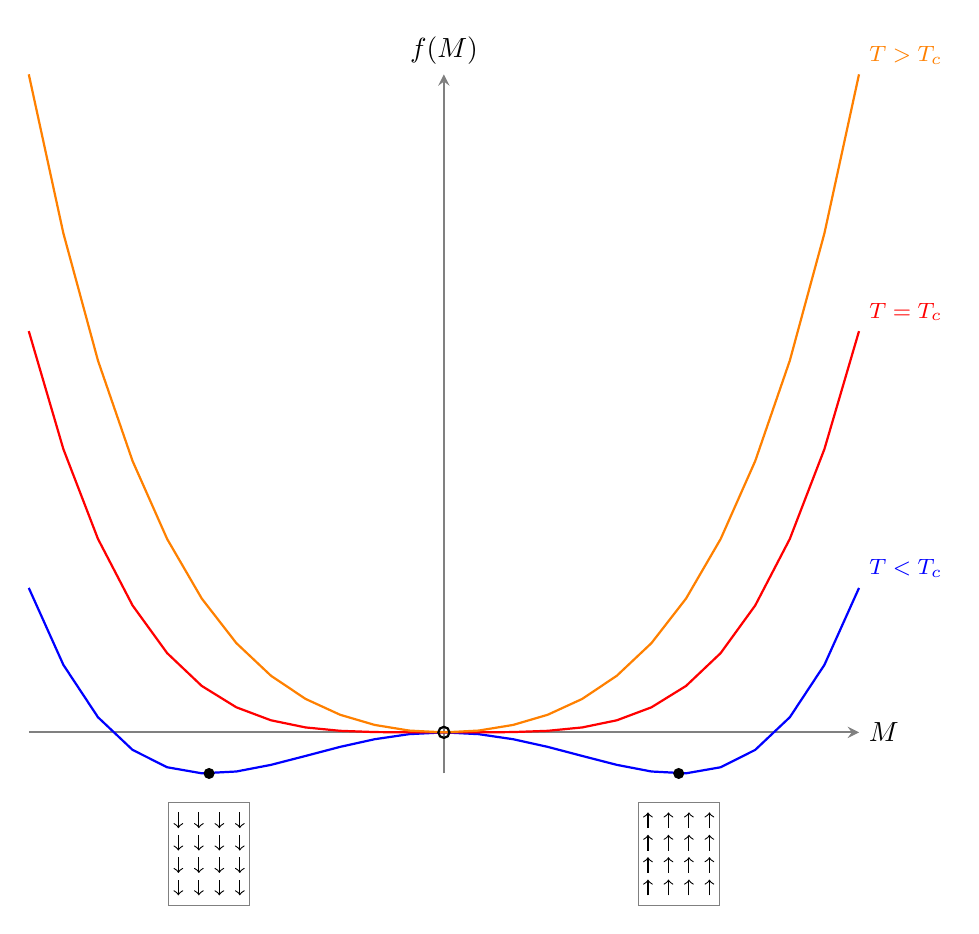
\begin{tikzpicture}[
        spins/.style={
          matrix,
          draw,
          gray,
          outer sep=2pt,
          column sep=7pt,
          row sep=2pt,
          node distance=5pt}]
        \begin{axis}[
          sketch plots,
          label at end,
          width=\columnwidth,
          xlabel={$M$},ylabel={$f(M)$},
          ticks=none,
          domain=-2.5:2.5
        ]
          \addplot+[blue] {-4*x^2 + x^4}
            node[above right] {\footnotesize $T<T_c$};
          \addplot+[red] {x^4}
            node[above right] {\footnotesize $T=T_c$};
          \addplot+[orange] {+4*x^2 + x^4}
            node[above right] {\footnotesize $T>T_c$};
          \draw[thick,black] (axis cs: 0,0) circle (2pt);
          \node (s1) at (axis cs: {-2^(1/2)},-4) {};
          \node (s2) at (axis cs: {+2^(1/2)},-4) {};
          \fill (s1) circle (2pt) (s2) circle (2pt);
        \end{axis}
        \def\up{\draw[black,->] (0,-0.1) -- (0,0.1);}
        \def\dn{\draw[black,<-] (0,-0.1) -- (0,0.1);}
        \node [spins,below=of s1] {
          \dn & \dn & \dn & \dn\\
          \dn & \dn & \dn & \dn\\
          \dn & \dn & \dn & \dn\\
          \dn & \dn & \dn & \dn\\
        };
        \node [spins,below=of s2] {
          \up & \up & \up & \up\\
          \up & \up & \up & \up\\
          \up & \up & \up & \up\\
          \up & \up & \up & \up\\
        };
      \end{tikzpicture}
    \end{figure}
  \end{columns}
\end{frame}

\begin{frame}{Pure states}
  \begin{itemize}
    \item \textit{E.g.} the ``up'' and ``down'' states of a ferromagnet
    \item Satisfy a \alert{clustering property}, \textit{i.e.} correlations
      vanish at long distances,
      \textit{e.g.}
      \begin{equation*}
        \av{S_i S_j} - \av{S_i}\av{S_j} \to 0
        \quad\text{as}\quad
        \abs{\vec{r}_i-\vec{r}_j}\to\infty
      \end{equation*}
    \item For arbitrary thermodynamic state $\rho$, \textit{e.g.}
      \begin{equation*}
        \av{S_i S_j}_{\rho} = \sum_{\alpha} W_{\alpha} \av{S_i S_j}_{\rho_{\alpha}}
      \end{equation*}
    \item ``Mixed states'' have more than one $W_{\alpha} > 0$
    \item Characterize broken symmetry
    \item \alert{What do pure states look like in spin glasses?}
  \end{itemize}
\end{frame}

\begin{frame}{Pure states in spin glasses}
  \begin{itemize}
    \item Complicated, random-looking (depend on $J_{ij}$)
    \item Can't ``select'' states with a uniform field as for FM
    \item \alert{How many pure states?} Competing theories\dots
  \end{itemize}
  \begin{columns}[t]
    \column{0.5\textwidth}
    \centering
    \begin{figure}
      \centering
      \pgfmathsetmacro{\x}{0.6}
      \pgfmathsetmacro{\y}{0.9}
      \begin{tikzpicture}
        \begin{axis}[
          sketch plots,label at end,
          width=\columnwidth,
          height=0.6\columnwidth,
          xmin=-1,xmax=1,
          ymin=0,ymax=1,
          xtick={-\x,\x},
          xticklabels={$-\qea$,$+\qea$},
          xtick align=outside,
          ytick=\empty,
          xlabel={$q$}, ylabel={$P(q)$},
        ]
          \addplot+ [ycomb] coordinates {(-\x,\y) (\x,\y)};
        \end{axis}
      \end{tikzpicture}
    \end{figure}
    Single-pair, \textit{e.g.} \structure{``droplet''}
    \column{0.5\textwidth}
    \centering
    \begin{figure}
      \centering
      \begin{tikzpicture}
  \pgfmathsetmacro{\x}{0.6}
  \pgfmathsetmacro{\y}{0.9}
  \pgfmathsetmacro{\a}{0.1}
  \pgfmathsetmacro{\b}{0.6}
  \begin{axis}[
    sketch plots,label at end,
    width=\columnwidth,
    height=0.6\columnwidth,
    xmin=-1,xmax=1,
    ymin=0,ymax=1,
    xtick={-\x,\x},
    xticklabels={$-\qea$,$+\qea$},
    xtick align=outside,
    ytick=\empty,
    xlabel={$q$}, ylabel={$P(q)$},
    enlarge y limits=false,
    every axis plot post/.append style={red}
  ]
    \addplot+[ycomb,forget plot] coordinates {(-\x,\y) (\x,\y)};
    \addplot+[domain=-\x:\x] {\a + \b*x^2};
  \end{axis}
\end{tikzpicture}

    \end{figure}
    Many-pairs, \textit{e.g.} replica symmetry breaking \alert{(RSB)}
  \end{columns}
\end{frame}


\subsection{``Metastate'' idea}

\begin{frame}{Chaotic size dependence}
  \begin{itemize}
    \item Occurs in RSB-like scenario \autocite{newman1992multiple}
    \item
      \alert{System does not settle into a unique
        state in any finite region in the thermodynamic limit}
    \item Equivalently, the state observed in a finite, small window dependends
      on boundary conditions, far-away bonds
  \end{itemize}
  \begin{figure}
    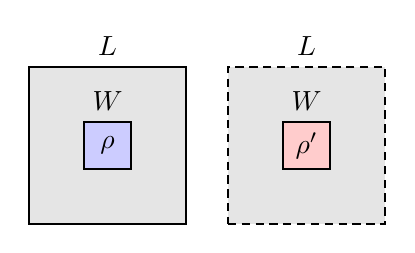
\begin{tikzpicture}
      \node (l1) [region=2cm,label=$L$] {};
      \node (w1) at (l1.center) [region=0.6cm,fill=blue!20,label=$W$] {$\rho$};
      \node (l2) [region=2cm,densely dashed,right=of l1,label=$L$] {};
      \node (w2) at (l2.center) [region=0.6cm,fill=red!20,label=$W$] {$\rho^{\prime}$};
    \end{tikzpicture}
  \end{figure}
  \alert{How can we describe the phase structure in the thermodynamic limit?}
\end{frame}

\begin{frame}{``Metastate'' idea}
  \begin{itemize}
    \item Probability distribution over thermodynamic states, $P(\rho)$
      \autocite{newman1997metastate}
    \item Defined as frequency of occurrence of a state $\rho$ in a finite
      window over all sequences of sizes and boundary conditions
    \item State observed is ``metastate-averaged state'' (MAS)
  \end{itemize}
  \begin{figure}
    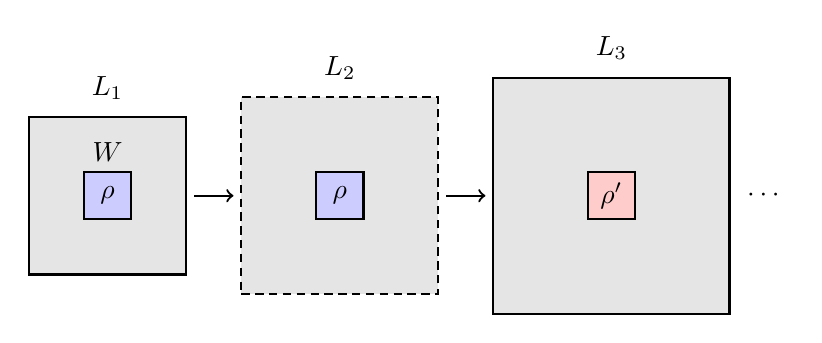
\begin{tikzpicture}
      \node (l1) [region=2cm,label=$L_1$,outer sep=1mm] {};
      \node (w1) at (l1.center) [region=0.6cm,fill=blue!20,label=$W$] {$\rho$};
      \node (l2) [region=2.5cm,densely dashed,right=of l1,outer sep=1mm,label=$L_2$] {}
        edge[<-] (l1);
      \node (w2) at (l2.center) [region=0.6cm,fill=blue!20] {$\rho$};
      \node (l3) [region=3cm,right=of l2,outer sep=1mm,label=$L_3$] {}
        edge[<-] (l2);
      \node (w3) at (l3.center) [region=0.6cm,fill=red!20] {$\rho^{\prime}$};
      \node at (l3.east) [anchor=west] {$\cdots$};
    \end{tikzpicture}
  \end{figure}
\end{frame}

\begin{frame}{Equivalent description of metastate}
  \begin{itemize}
    \item \textcite{aizenman1990rounding}
    \item Study correlations in a \alert{small window} $W$
    \item Average over \alert{distant bonds} between $M$ and $L$
    \item $W \ll M \ll L$
  \end{itemize}
  \begin{figure}
    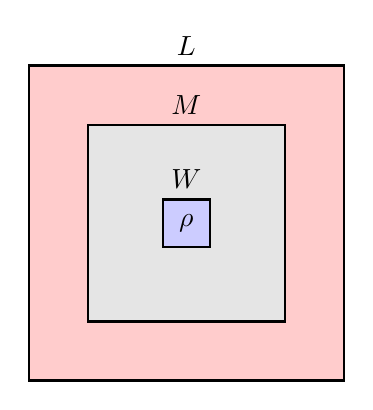
\begin{tikzpicture}
      \node (l) [region=4cm,fill=red!20,label=$L$,outer sep=0] {};
      \node (m) [region=2.5cm,label=$M$,outer sep=0] {};
      \node (w) [region=0.6cm,fill=blue!20,label=$W$] {$\rho$};
    \end{tikzpicture}
  \end{figure}
\end{frame}

\begin{frame}{Decay of correlations (static calculation)}
  Performing metastate average of (spin-glass) correlations in a small window,
  find
  \begin{itemize}
    \item If only a \alert{single pair} of pure states
    \begin{equation*}
      \av{S_i S_j}^2_{\text{MAS}} = \text{constant}
    \end{equation*}
    \item If there are \alert{many pairs}
    \begin{equation*}
      \av{S_i S_j}^2_{\text{MAS}} \propto r_{ij}^{-\alpha_s}
    \end{equation*}
    \item For $d>6$ (mean-field regime) get from RSB theory%
      \footnote{\textcite{read2014short}}
      \begin{equation*}
        \boxed{\alpha_s = d-4}
      \end{equation*}
  \end{itemize}
\end{frame}


\subsection{Dynamical correlations}

\begin{frame}{Dynamical correlations}
  Dynamical correlation function
  \begin{equation*}
    C_4(r,t) \equiv \dav{\av{S_i S_j}^2_t}
  \end{equation*}
  From simulations of short-range models at $T<T_c$:
  \begin{itemize}
    \item Following a quench, fluctuations equilibrate up to scale $\xi(t)$,
      \emph{dynamical correlation length}
      \begin{equation*}
        \xi(t) \sim t^{1/z(T)}
      \end{equation*}
    \item At distances less than $\xi(t)$, observe \alert{power law decay} of
      correlations
    \item Scaling hypothesis
    \begin{equation*}
        C_4(r,t) = r_{ij}^{-\alpha_d} f\del{\frac{r}{\xi(t)}}
    \end{equation*}
  \end{itemize}
  \alert{Are the static and dynamic exponents equal, $\alpha_d=\alpha_s$?}
\end{frame}


\subsection{Numerical methods}

\begin{frame}{Method}
  To make connection with exact result, need $d>6$. But simulation of spin
  glasses for large $d$ is \emph{hard}\dots
  \begin{itemize}
    \item Need range of sizes to study $L$ dependence, but $N=L^d$
    \item (Equilibrium) simulations limited to about $N=10^4$
  \end{itemize}
  Instead, study \alert{one-dimensional} models with \alert{long-range}
  interactions
  \begin{itemize}
    \item Bond strength falls off as a power of distance
      \begin{equation*}
        \dav{J_{ij}^2} \propto R_{ij}^{-2\sigma}
      \end{equation*}
    \item Correspondence between $d$ and $\sigma$ (for $d>6$, $T=T_c$)
      \begin{equation*}
        \boxed{d_{\text{eff}} = \frac{2}{2\sigma - 1}}
      \end{equation*}
  \end{itemize}
  We choose \alert{$\sigma=5/8$} (corresponding to \alert{$d=8$})
\end{frame}

\begin{frame}{Diluted model}
  Simulation of long-range model inefficient: $\mathcal{O}(N^2)$ update

  Instead, study \alert{diluted model\footnote{\textcite{leuzzi2008dilute}}}
  \begin{itemize}
    \item Each spin interacts with $z_b$ neighbors ($z_b=6$ here)
    \item Power-law decay of bond \alert{probability}
    \item When bond exists, drawn from Gaussian distribution with unit variance
      (independent of distance)
      \begin{equation*}
        P(J_{ij}) = (1-p_{ij})\delta(J_{ij}) +
        \frac{p_{ij}}{\sqrt{2\pi}} e^{-J_{ij}^2/2},\quad
        p_{ij} \sim R_{ij}^{-2\sigma}
      \end{equation*}
    \item Relatively efficient $\mathcal{O}(N z_b)$ update
  \end{itemize}
\end{frame}


\subsection{Results}

\begin{frame}{Results}
  \begin{columns}
    \column{0.5\textwidth}
    Large-scale Monte Carlo simulation
    \begin{itemize}
      \item Strong finite-size effects
      \item Data saturate at largest size studied, $N=2^{26}$
    \end{itemize}
    \alert{$\alpha_d=\alpha_s$?}
    \begin{itemize}
      \item For 1D model $R$ is effective volume,
        $R \sim r^{d_{\text{eff}}}$, so\footnotemark
        \begin{align*}
          r^{\alpha_s}
          &\equiv r^{-(d-4)} \\
          &\sim R^{-(d_{\text{eff}}-4)/d_{\text{eff}}} \\
          &= R^{-(3-4\sigma)}
        \end{align*}
    \end{itemize}
    \column{0.5\textwidth}
    \begin{tikzpicture}
  \begin{loglogaxis}[
    name=plot,
    width=\columnwidth,
    height=\columnwidth,
    font=\scriptsize,
    mark size=1.5pt,
    xmin=1,xmax=10^5,ymin=10^-5,
    xlabel={$R$},
    ylabel={$C_4(R,t)$},
    with y errors,
    mark options={fill opacity=0.4},
    legend pos=south west,
    legend style={font=\tiny},
    legend image code/.code={
      \draw[mark repeat=2,mark phase=2]
      plot coordinates {
        (0cm,0cm)
        (0.15cm,0cm)        %% default is (0.3cm,0cm)
        (0.3cm,0cm)         %% default is (0.6cm,0cm)
      };
    }
  ]
    \foreach \n in {10,14,18,22,26} {
      \addplot table[x=r,y=mean,y error=sem] {data/c4-vs-r-n\n.csv};
      \addlegendentryexpanded{$N=2^{\n}$}
    }
    \node [draw,anchor=north east] at (rel axis cs: 0.97,0.97){%
      $\begin{aligned}
        \sigma &= 5/8 \\
        t &= 2^{14}
      \end{aligned}$};
  \end{loglogaxis}
\end{tikzpicture}

  \end{columns}
  \footnotetext{\textcite{banos2012correspondence}}
\end{frame}

\begin{frame}{Results: dynamical correlations}
  \begin{figure}
    \centering
    \begin{tikzpicture}
  \pgfmathdeclarefunction{f1}{1}{\pgfmathparse{0.23*#1^(-0.5 )}}
  \pgfmathdeclarefunction{f2}{1}{\pgfmathparse{2.8 *#1^(-1.25)}}
  \def\pad#1{\ifnum#1<10 0#1\else#1\fi}
  \def\filename{data/c4-vs-r-t\pad{\logtime}.csv}
  \def\logtimes{4,6,8,10,12,14}

  \begin{loglogaxis}[
    width=0.7\textwidth,
    xmin=1,xmax=10^5,
    ymin=10^-5,ymax=1,
    xlabel={$R$},
    ylabel={$C_4(R,t)$},
    font=\footnotesize,
    legend pos=south west,
    legend cell align=left,
  ]

    \foreach \logtime in \logtimes {%
      \addplot+[only marks, with y errors] table[
        x=r,
        y=C4_mean,
        y error=C4_sem
      ] {\filename};
      \addlegendentryexpanded{$t=2^{\logtime}$}
    }

    \addplot [domain=1:10^5, samples=2] {f1(x)}
      node [above, pos=0.7, sloped] {$-(3-4\sigma)$};
    \addplot [densely dashed, domain=1:10^5, samples=2] {f2(x)}
      node [above, pos=0.2, sloped] {$-2\sigma$};

    \node [draw, anchor=north east] at (rel axis cs: 0.97,0.97){%
      $\begin{aligned}
        \sigma &= 5/8 \\
        N &= 2^{26}
      \end{aligned}$};
  \end{loglogaxis}
\end{tikzpicture}

    \begin{tabular}{ll}
      \alert{Short distance, long time:} &
        \alert{slope $\approx -1/2 = 3-4\sigma=\alpha_s$} \\
      Long distance, short time: &
        slope $\approx -5/4 = -2\sigma$
    \end{tabular}
  \end{figure}
\end{frame}

\begin{frame}{Results: dynamical correlations (2)}
  \begin{figure}
    \centering
    \begin{tikzpicture}
  \def\sigmafrac{5/8}
  \def\zT{1.4}
  \def\pad#1{\ifnum#1<10 0#1\else#1\fi}
  \def\filename{data/c4-vs-r-t\pad{\logtime}.csv}
  \def\logtimes{4,6,8,10,12,14}

  \pgfmathsetmacro\sigmaval{\sigmafrac}
  \pgfmathdeclarefunction{xi}{1}{\pgfmathparse{#1^(1/\zT)}}

  \begin{semilogxaxis}[
    width=0.7\textwidth,
    xmin=1,xmax=255,
    ymin=-1,ymax=-0.45,
    xlabel=$R$,
    ylabel=$\alpha_{\text{eff}}$,
    ytick={-1.0,-0.9,...,-0.4},
    font=\footnotesize,
    legend pos=outer north east
  ]
    \foreach \logtime in \logtimes {%

      \addplot+[mark=none,smooth,forget plot,raw gnuplot] gnuplot {
        set datafile separator ",";
        set logscale x;
        set samples 20;
        f(x) = a + b*x + c*x**2;
        fit f(x) '\filename' every ::4 using (log($3)):6:7 via a,b,c;
        plot [x=1:255] f(log(x));
      };
      \addplot+[
        only marks,
        with y errors,
      ] table [
        x=r,
        y=alpha_mean,
        y error=alpha_sem
      ] {\filename};
      \addlegendentryexpanded{$t=2^{\logtime}$}
    }
    \addplot [dashed,domain=1:255,samples=2] {-0.5};
    \node [draw,anchor=south west] at (rel axis cs: 0.03,0.03){%
      $\begin{aligned}
        \sigma &= 5/8 \\
        N &= 2^{26} \\
        z &= 1.4
      \end{aligned}$};
  \end{semilogxaxis}
\end{tikzpicture}

  \end{figure}
\end{frame}

\begin{frame}[fragile]{Results: scaling collapse}
  \begin{columns}
    \column{0.45\textwidth}
    Scaling hypothesis
    \begin{equation*}
      C_4(R,t)=R^{-(3-4\sigma)} f\del{\frac{R}{\xi(t)}}
    \end{equation*}
    assuming
    \begin{equation*}
      \xi(t) \propto t^{1/z(T)}
    \end{equation*}
    Find good collapse with
    \begin{equation*}
      z(T) = 1.4(1)
    \end{equation*}
    \column{0.55\textwidth}
    \begin{figure}
      \begin{tikzpicture}
  \def\sigmafrac{5/8}
  \def\zT{1.4}
  \def\pad#1{\ifnum#1<10 0#1\else#1\fi}
  \def\filename{data/c4-vs-r-t\pad{\logtime}.csv}
  \def\logtimes{4,6,8,10,12,14}
  \pgfmathsetmacro\sigmaval{\sigmafrac}
  \pgfmathdeclarefunction{xi}{1}{\pgfmathparse{#1^(1/\zT)}}
  \pgfplotsset{every axis/.append style={mark options={fill opacity=0.4}}}

  \begin{loglogaxis}[
    name=plot,
    width=\columnwidth,
    height=\columnwidth,
    xmin=10^-3,xmax=2000,
    ymin=10^-3,ymax=0.3,
    xlabel={$R/\xi(t)\,\left(=R/t^{1/z(T)}\right)$},
    ylabel={$R^{3-4\sigma} C_4(R,t)$},
    font=\footnotesize,
    xlabel near ticks,ylabel near ticks,
    legend pos=south west,
    legend cell align=left
  ]
    \foreach \logtime in \logtimes {%
      \addplot+[only marks, with y errors] table[
        x expr=\thisrow{r}/xi(2^\logtime),
        y expr=\thisrow{r}^(3-4*\sigmaval)*\thisrow{C4_mean},
        y error expr=\thisrow{r}^(3-4*\sigmaval)*\thisrow{C4_sem}
      ]{\filename};
      \addlegendentryexpanded{$t=2^{\logtime}$}
    }
  \end{loglogaxis}
  \matrix[
    matrix of nodes,
    inner sep=2pt,
    outer sep=1ex,
    column sep=1ex,
    font=\footnotesize,anchor=south
  ]
    at (plot.north) {
    $\sigma=5/8$ &
    $N=2^{26}$ &
    \alert{$z(T)=1.4$} \\
  };
\end{tikzpicture}

    \end{figure}
  \end{columns}
\end{frame}

\begin{frame}{Summary}
  \begin{itemize}
  \item
    Nonequilibrium dynamics of a model in the mean-field regime appears
    to be consistent with predictions of the metastate in the RSB scenario.
    \item 
      Assuming $1/z(T) \propto T$, predict $z(T_c)=4.5(6)$ for $d=8$ SR model
      (consistent with mean-field $z_c$)
    \item Results suggest
    \begin{itemize}
      \item RSB is a useful description of the spin glass phase in the
        mean-field regime, $d>6$
      \item The dynamic and static metastates are equivalent (at least in this regime)
    \end{itemize}
  \end{itemize}
\end{frame}


\section{Nonextensive spin glasses}

\subsection{Nonextensive regime}

\begin{frame}{Nonextensive regime}
  \begin{itemize}
    \item For 1DLR model
    \begin{equation*}
      \dav{J_{ij}^2} \propto \frac{1}{R_{ij}^{2\sigma}}
    \end{equation*}
    \item Free energy grows faster than $N$ if $\sigma<1/2$, in particular
      \begin{equation*}
        T_c^{\text{MF}} = \sum_j \dav{J_{ij}^2} \to \infty
        \quad\text{as}\quad
        \sigma \to (1/2)^+
      \end{equation*}
    \item Need to rescale interactions to preserve $N\to\infty$ limit
      \begin{equation*}
        \dav{J_{ij}^2} = \frac{c(\sigma)}{R_{ij}^{2\sigma}}
      \end{equation*}
    \item Choose convention
      \begin{equation*}
        T_c^{\text{MF}} \equiv 1,\quad
        c(\sigma) = \del{\sum_j R_{ij}^{-2\sigma}}^{-1}
      \end{equation*}
  \end{itemize}
\end{frame}

\begin{frame}{Nonextensive regime (2)}
  \begin{equation*}
    \dav{J_{ij}^2} \propto \frac{1}{R_{ij}^{2\sigma}},\quad
    T_c^{\text{MF}} \equiv 1
  \end{equation*}
  \begin{itemize}
    \item $\sigma \to 1/2$ from above corresponds to $d \to \infty$
      \begin{equation*}
        d_{\text{eff}} = \frac{2}{2\sigma - 1}
      \end{equation*}
    \item $\sigma=0$ corresponds to the mean-field (SK) model
    \item Mean-field \emph{critical exponents} for $\sigma<2/3$ ($d>6$)
  \end{itemize}
  \alert{Is the (detailed) behavior mean-field-like everywhere in the
    nonextensive regime ($0 \leq \sigma \leq 1/2$)?}
  \autocite{mori2011instability}
  \begin{itemize}
    \item Previously demonstrated for the ferromagnet, \textit{e.g.}
      \textcite{cannas2000evidence}
    \item Check for spin glasses\dots
  \end{itemize}
\end{frame}


\subsection{Numerical methods}

\begin{frame}{Parallel-tempering Monte Carlo}
  \alert{Slow dynamics} makes Monte Carlo difficult. Systems at low
  temperature often get stuck in metastable states.

  \alert{Parallel tempering} helps with this\dots
  \begin{itemize}
    \item Simulate many identical systems (replicas) simultaneously over a
      range of temperatures
    \item Replicas perform a random walk in temperature space
  \end{itemize}
  \begin{figure}
    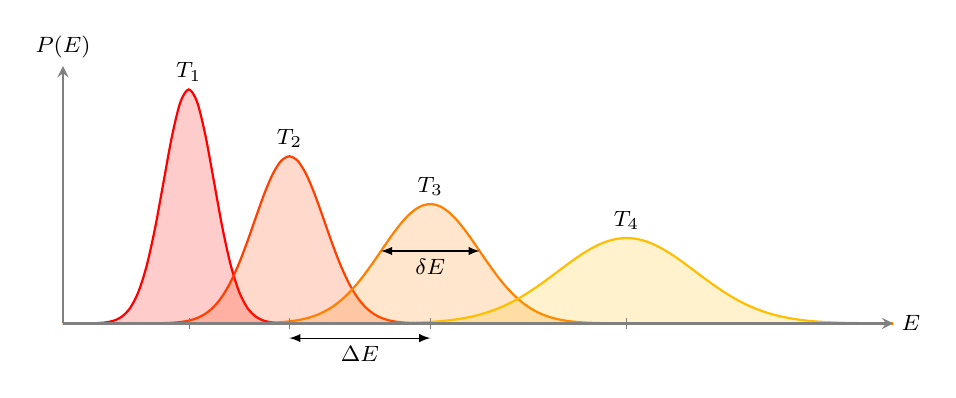
\begin{tikzpicture}
  \footnotesize
  \def\energies{{1,1.4,1.96,2.74}}
  \begin{axis}[
    label at end,
    width=\columnwidth,
    height=0.4\columnwidth,
    xlabel={$E$},ylabel={$P(E)$},
    xtick={1,1.4,1.96,2.74},
    xticklabel=\empty,
    ytick=\empty,
    axis lines=left,
    axis on top,
    enlarge y limits=upper,
    clip=false,
    no marks,
    samples=100,
    domain=0.5:3.8,
    smooth,
    every axis plot/.append style={fill opacity=0.2}
  ]
    \foreach [count=\i] \clr in {red,red!50!orange,orange,orange!50!yellow} {
      \pgfmathsetmacro\en{\energies[\i-1]}
      \edef\temp{%
        \noexpand\addplot+[\clr, fill=\clr] {gauss(x, \en, 0.1*\en)};
        \noexpand\node[above] at (\en, {gauss(\en,\en,0.1*\en)}) {$T_{\i}$};
      }
      \temp
    }
    \pgfmathsetmacro\ena{\energies[1]}
    \pgfmathsetmacro\enb{\energies[2]}
    \draw [latex-latex]
      (axis cs: \ena, -0.25) --
        node [below] {$\Delta E$}
      (axis cs: \enb, -0.25);
    \draw [latex-latex]
      (axis cs: 0.9*\enb, {gauss(0.9*\enb,\enb,0.1*\enb)}) --
        node [below] {$\delta E$}
      (axis cs: 1.1*\enb, {gauss(1.1*\enb,\enb,0.1*\enb)});
  \end{axis}
\end{tikzpicture}

  \end{figure}
\end{frame}

\begin{frame}{Method}
  \begin{itemize}
    \item Measure \alert{Binder ratio}
    \begin{equation*}
      g \equiv \frac{1}{2}\del{3 - \frac{\dav{\av{q^4}}}{\dav{\av{q^2}}^2}}
    \end{equation*}
    \item $g \to 1$ at low temperatures, $g \to 0$ at high temperatures
    \item Finite-size scaling for $d>6$
      \begin{equation*}
        g(L,T) \sim \widetilde{g}\sbr{L^{1/3} (T-T_c)}
      \end{equation*}
    \item No size dependence at $T=T_c$
  \end{itemize}
  \alert{Determine $T_c$ from the intersection of data for $g$ for different sizes}
\end{frame}


\subsection{Results}

\begin{frame}{Results: $\sigma=0.25$, Binder ratio}
  \centering
  \begin{tikzpicture}
  \def\sig{25}
  \def\pad#1{\ifnum#1<10 0#1\else#1\fi}
  \def\filename{data/binder-c-s\sig-l\pad{\logsize}.csv}
  \def\logsizes{6,7,8,9,10,11,12}
  \def\xmin{0.8}
  \def\xmax{1.2}
  \def\ymin{0}
  \def\ymax{0.6}
  \def\tc{1}
  \begin{axis}[
    width=0.7\textwidth,
    xmin=\xmin,xmax=\xmax,ymin=\ymin,ymax=\ymax,
    xlabel={$T$},
    ylabel={$g$},
    extra x ticks={\tc},
    extra x tick style={xticklabel=\empty, grid=major},
    legend pos=outer north east,
    legend cell align=left,
    legend style={font=\footnotesize},
  ]
    \foreach \logsize in \logsizes {%
      \addplot+[with y errors] table [
        x=T,
        y=mean,
        y error=sem
      ] {\filename};
      \addlegendentryexpanded{$L=2^{\logsize}$}
    }
  \end{axis}
\end{tikzpicture}

  \begin{equation*}
    T^*(L,2L) = T_c + \frac{A}{L^{2/3}} + \cdots
  \end{equation*}
\end{frame}

\begin{frame}{Results: $\sigma=0.25$, intersection temperatures}
  \centering
  \begin{figure}
    \begin{tikzpicture}
  \def\Tcg{1.007}
  \def\TcX{1.002}
  \def\Tcgerr{1.007(4)}
  \def\TcXerr{1.002(1)}
  \def\Ag{-1.66}
  \def\AX{-0.266}
  \begin{axis}[
    name=plot,
    width=0.7\textwidth,
    xlabel={$L^{-2/3}$},
    ylabel={$T^*(L,2L)$},
    extra y ticks=1,
    extra y tick style={yticklabel=\empty,grid=major},
    enlarge x limits=false
  ]
    % plot data
    \pgfplotstableread{data/Tx-c-s25.csv}\data

    \addplot+[with y errors,only marks] table [
      x expr=\thisrow{L}^(-2/3),
      y=Tx_chi_mean,
      y error=Tx_chi_std,
    ] {\data};
    \label{plot:chi-c-s25}

    \addplot+[with y errors,only marks] table [
      x expr=\thisrow{L}^(-2/3),
      y=Tx_G_mean,
      y error=Tx_G_std,
    ] {\data};
    \label{plot:binder-c-s25}

    % plot fit lines
    \addplot+[mark=none,samples=2,domain=0:0.07] { \TcX + \AX*x };
    \addplot+[mark=none,samples=2,domain=0:0.07] { \Tcg + \Ag*x };

    % make table of fit parameters
  \end{axis}
  \matrix[
    matrix of nodes,
    anchor=south west,
    outer sep=5pt,
    row sep=0,
    nodes={anchor=west},
    font=\footnotesize
  ] at at (plot.south west) {
      & $T^*(\infty)$ \\
      \ref{plot:chi-c-s25} $\chi_{\text{SG}}/L^{1/3}$ & $\TcXerr$ \\
      \ref{plot:binder-c-s25} $g$ & $\Tcgerr$ \\
  };
\end{tikzpicture}

  \end{figure}
  \alert{Consistent with mean-field (SK) result $T_c^{\text{MF}}=1$}
\end{frame}

\begin{frame}{Results: $\sigma=0.375$, diluted model}
  \centering
  \begin{figure}
    \begin{tikzpicture}
  \def\Tcg{2.060}
  \def\TcX{2.054}
  \def\Tcgerr{2.060(5)}
  \def\TcXerr{2.054(2)}
  \def\Ag{-5.28}
  \def\AX{-1.30}
  \begin{axis}[
    name=plot,
    width=0.7\textwidth,
    xlabel={$L^{-2/3}$},
    ylabel={$T^*(L,2L)$},
    extra y ticks=2.056,
    extra y tick style={yticklabel=\empty,grid=major},
    enlarge x limits=false
  ]
    % plot data
    \pgfplotstableread{data/Tx-d-s38.csv}\data

    \addplot+[with y errors,only marks] table [
      x expr=\thisrow{L}^(-2/3),
      y=Tx_chi_mean,
      y error=Tx_chi_std,
    ] {\data};
    \label{plot:chi-c-s25}

    \addplot+[with y errors,only marks] table [
      x expr=\thisrow{L}^(-2/3),
      y=Tx_G_mean,
      y error=Tx_G_std,
    ] {\data};
    \label{plot:binder-c-s25}

    % plot fit lines
    \addplot+[mark=none,samples=2,domain=0:0.03] { \TcX + \AX*x };
    \addplot+[mark=none,samples=2,domain=0:0.03] { \Tcg + \Ag*x };

    % make table of fit parameters
  \end{axis}
  \matrix[
    matrix of nodes,
    anchor=south west,
    outer sep=5pt,
    row sep=0,
    nodes={anchor=west},
    font=\footnotesize
  ] at at (plot.south west) {
      & $T^*(\infty)$ \\
      \ref{plot:chi-c-s25} $\chi_{\text{SG}}/L^{1/3}$ & $\TcXerr$ \\
      \ref{plot:binder-c-s25} $g$ & $\Tcgerr$ \\
  };
\end{tikzpicture}

  \end{figure}
  \alert{Consistent with mean-field (Viana-Bray) result $T_c^{\text{MF}} \approx 2.056$}
\end{frame}

\section*{Summary}

\begin{frame}{Summary}

  \begin{itemize}
  \item
    Monte Carlo results for the transition temperature for undiluted and
    diluted models for several values of $\sigma$ in the nonextensive regime
    ($0 \leq \sigma < 1/2$) are \alert{consistent with mean-field predictions.}
  \item
    Strong evidence that the detailed behavior (\textit{i.e.} not just critical
    exponents) of nonextensive models is given by mean-field theory
  \end{itemize}
\end{frame}

\section*{Acknowledgements}

\begin{frame}{Acknowledgements}
  \begin{itemize}
    \item Peter Young
    \item Sriram Shastry and Josh Deutsch
    \item Itay Hen
    \item Helmut Katzgraber, Burcu Yucesoy, Jon Machta
    \item NSF, for funding the research
    \item Maria Sliwinski, Michele Yoskovich, Davina Walker, Jennifer Raab
    \item Friends and fellow grad students
    \pause
    \item You, the audience!
  \end{itemize}
  \centering\Huge
  Thank you!
\end{frame}

\end{document}


